\documentclass[a4paper,12pt]{article}
\usepackage[spanish]{babel}
\textheight = 25cm 
\textwidth = 18cm
\topmargin = -2cm 
\oddsidemargin = -1.0cm
\usepackage[utf8]{inputenc}
\usepackage{amsmath}
\usepackage{amsfonts}
\usepackage{amssymb}
\usepackage{graphicx}
\usepackage{parskip}
\usepackage[dvipsnames]{xcolor}
\usepackage{xcolor}
\usepackage{float}
\usepackage{siunitx}
\usepackage{changepage}
\usepackage{subcaption}
\usepackage{enumerate}
\usepackage{cite}
\usepackage{url}
\usepackage{hyperref}
\usepackage[export]{adjustbox}
\decimalpoint
\usepackage{colortbl}
\setlength{\arrayrulewidth}{.2mm}
\setlength{\tabcolsep}{2pt}
\usepackage{listings}

\newcommand{\der}[2]{\frac{d #1}{d #2}}
\newcommand{\dder}[2]{\frac{d^{2} #1}{d^{2} #2}}
\newcommand{\pder}[2]{\frac{\partial#1}{\partial#2}}
\newcommand{\ppder}[2]{\frac{\partial^2#1}{\partial#2^2}}

\newcommand{\grad}[1]{\nabla#1}
\newcommand{\diver}[1]{\nabla \cdot #1}
\newcommand{\rot}[1]{\nabla \times #1}

\newcommand{\parent}[1]{\left( #1 \right)}
\newcommand{\corch}[1]{\left[ #1 \right]}

\newcommand{\R}{\mathbb{R}}
\newcommand{\N}{\mathbb{N}}
\newcommand{\C}{\mathbb{C}}
\newcommand*\dif{\mathop{}\!\mathrm{d}}


\begin{document}
\title{
\textbf {Algoritmos Computacionales}\\ \textsc{Proyecto intermedio}\\
\textcolor{Blue}{Facultad de Ciencias, UNAM}
\author{
Diego Alberto Barceló Nieves\\
Mauricio Sandoval Cuenca\\
Juan Pablo Gamucero Arana
}
\date{}
}
\begin{minipage}[left]{3cm}
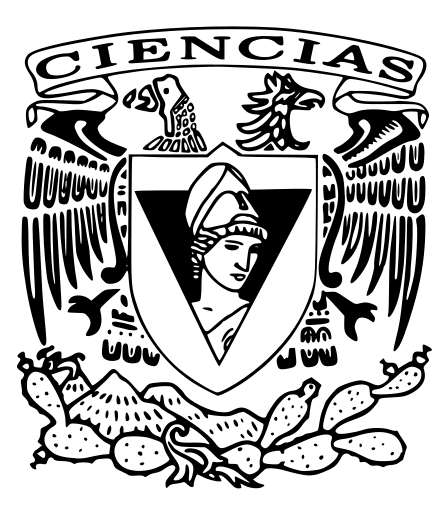
\includegraphics[width=3cm]{img/EscudoCiencias.png}
\end{minipage}
\begin{minipage}[c]{11.8cm}
\maketitle
\end{minipage}
\begin{minipage}[right]{3cm}
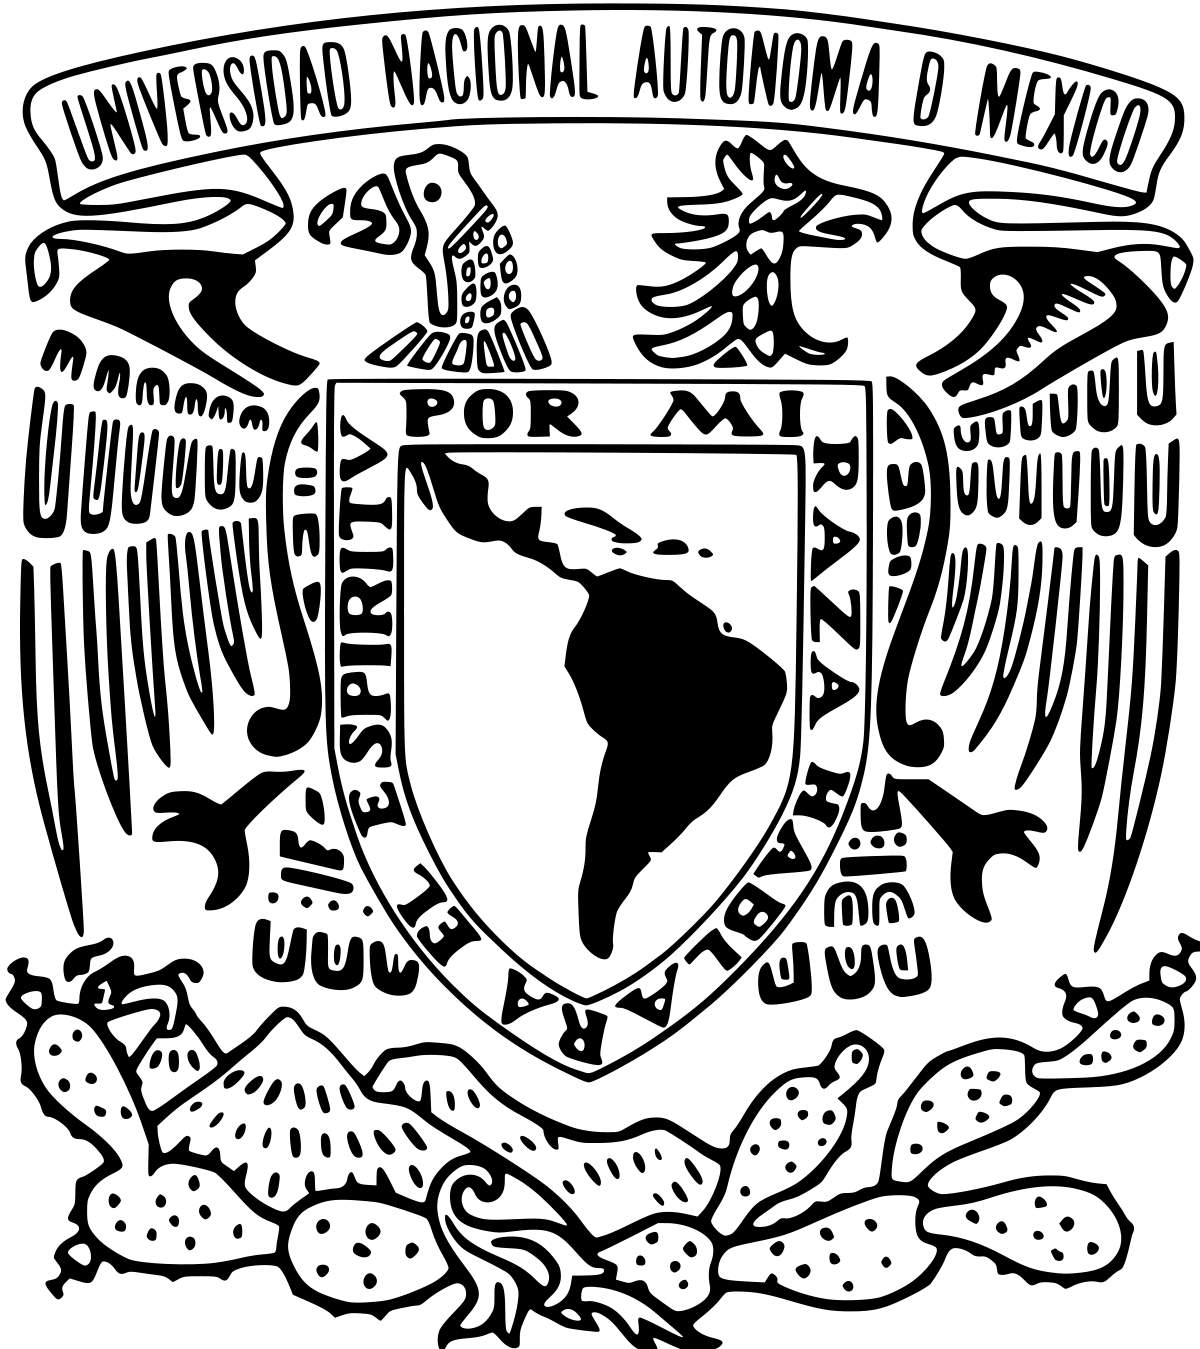
\includegraphics[width=3cm]{img/escudoUNAM.png}
\end{minipage}
{\color{gray}\hrule} 

\textbf{Instrucciones:}
Elige 2 de los 4 ejercicios que se muestran a continuación y entrega las soluciones en un notebook con código de Julia. 

\section*{Ejercicio 1: Aproximación de $\pi$}

Una forma para estimar el valor de $\pi$ ($3.141592...$) es usando el método de Monte Carlo. Primero, tomamos un cuadrado de 1 $\times$ 1 y un círculo inscrito de radio $\frac{1}{2}$, generamos una cantidad arbitraria de puntos uniformemente distribuidos sobre la superficie del cuadrado y coloreamos de rojo aquellos que se encuentren sobre la superficie del círculo, y de azul, aquellos que estén fuera  (ver Figura \ref{fig:pi}).

\begin{figure}[h!]
    \centering
    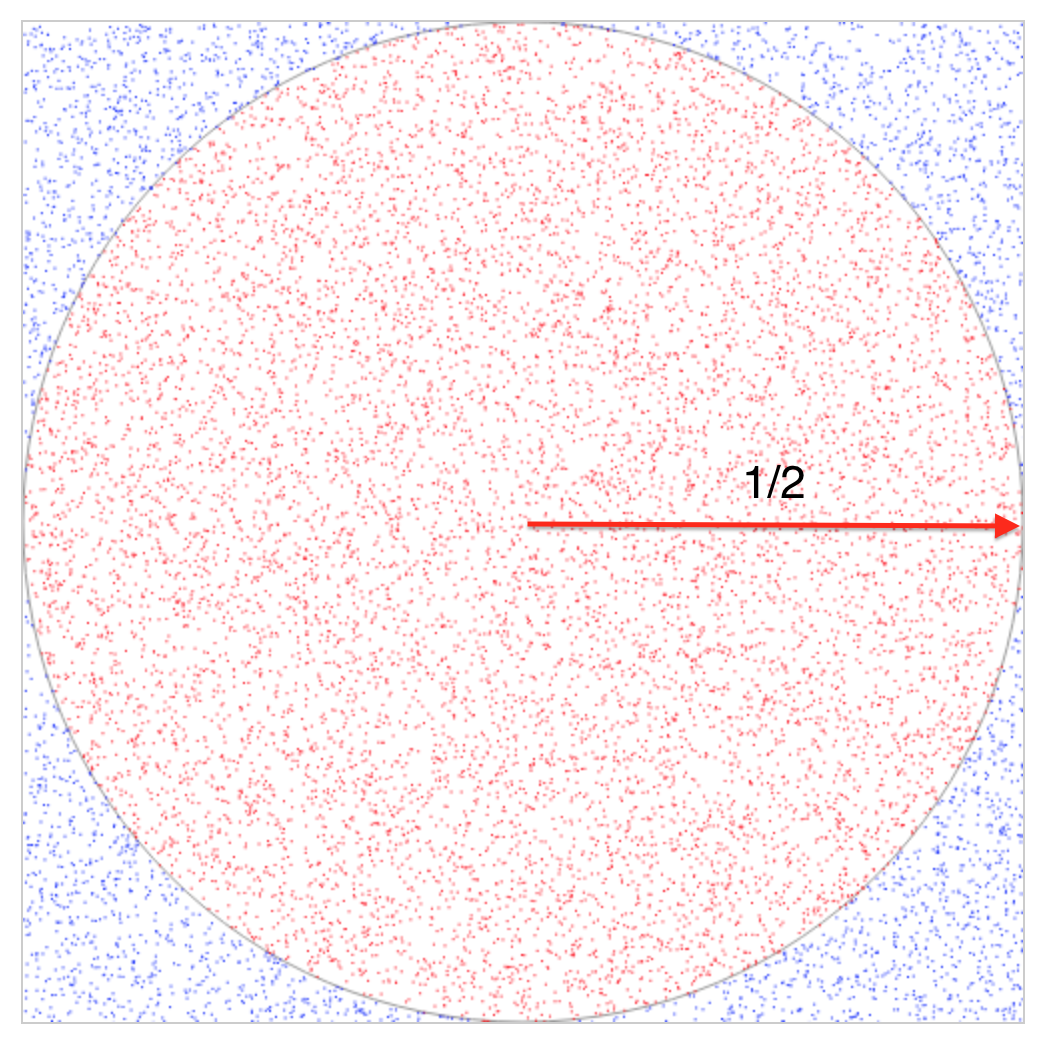
\includegraphics[width=.4\linewidth]{img/pi.png}
    \caption{Aproximación de $\pi$ por el método de Monte Carlo}
    \label{fig:pi}
\end{figure}

Ahora, tenemos que el área del círculo esta dada por $\pi r^2 = \frac{\pi}{4}$, mientras que el área del cuadrado es igual a $1$ por lo que, si dividimos el área del círculo entre el área del cuadrado, obtenemos $\frac{\pi}{4}$. Además, si $N_{rojo}$ es el número de puntos rojos y $N_{total}$ es el número total de puntos, entonces $\frac{N_{rojo}}{N_{total}}$ es una aproximación del cociente de las áreas para $N_{total}$ lo suficientemente grande; en otras palabras,
\[
    \frac{\pi}{4} \approx \frac{N_{rojo}}{N_{total}},
\] 
de donde se sigue que
\begin{equation}\label{eq: Monte Carlo}
    \pi \approx 4\ \frac{N_{rojo}}{N_{total}}.
\end{equation}
    
\noindent La ecuación (\ref{eq: Monte Carlo}) nos da la estimación de $\pi$ por el método Monte Carlo.

\begin{enumerate}
    \item Escribe un algoritmo que estime el valor de $\pi$ y que te permita visualizar algo similar al gráfico de la Figura \ref{fig:pi}, asegúrate de incluir el conteo del número de puntos rojos, número de puntos totales, y la respectiva estimación de $\pi$ (\textbf{6 puntos}).
    \item En promedio\footnote{Al tratarse de un método aleatorio, los resultados variarán de una ejecución a otra, por eso es importante tomar el promedio u otro estadístico.}, ¿cuántos puntos necesitas generar para obtener una precisión de $\pm 0.01$? (\textbf{2 puntos})
    \item Realiza una gráfica del error de la estimación en función del número de puntos comparando contra el valor predeterminado de $\pi$ de Julia (que se obtiene llamando a la constante \texttt{pi}) (\textbf{2 puntos}).
\end{enumerate}
\newpage
\section*{Ejercicio 2: Rana saltarina}
Una rana saltarina necesita atravesar un río para
llegar a su hogar. La rana inicia en la orilla izquierda del río, y su camino consiste en una
secuencia de rocas etiquetadas con los números $1, 2, 3, 4 
\dots, n-1$; hasta la orilla derecha del río, etiquetada con $n$. Todas las rocas adyacentes están espaciadas en una unidad de distancia, al igual que la roca $n-1$ de la orilla derecha y la orilla izquierda de la roca $1$. Es decir, a la rana le toma $n$ saltos de una unidad llegar hasta la otra orilla, aunque
su recorrido está sujeto a las siguientes restricciones:

    \begin{itemize}
        \item La rana solo puede dar saltos de longitud
        $1$ o $2$ unidades de longitud. 
        \item La rana no puede retroceder. 
    \end{itemize}
    
¿De cuántas formas distintas puede la rana saltarina
atravesar el río dado un valor de $n$?

    \begin{enumerate}
        \item Diseña un algoritmo que resuelva este 
        problema y represéntalo en pseudocódigo
        o diagrama de flujo (\textbf{3 puntos}).
        \item Implementa este algoritmo en Julia. La 
        idea es que tu programa reciba un entero $n$
        (el tamaño del río), y devuelva $N$, el número
        de formas distintas que la rana puede cruzar
        (\textbf{5 puntos}). 

        Tu programa será aceptado si devuelve el valor correcto
        de $N$ para cada valor de $n$, con $1\leq n\leq 45$
        \item Reflexiona sobre la complejidad temporal
        y espacial de tu algoritmo. ¿Cómo cambia el tiempo
        de ejecución de tu programa conforme crece $n$?, 
        ¿cómo cambia el espacio ocupado en la memoria de 
        la máquina conforme incrementa $n$?
        (\textbf{1 punto})
        \item Reflexiona sobre el valor máximo que 
        puede tomar $n$ de tal forma que no haya
        \textit{sobreflujo} en tus resultados de $N$
        (\textbf{1 punto}).
    \end{enumerate}

    \textit{Ejemplo 1}
    \begin{verbatim}
        Entrada: n=2
        Salida: 2
        Explicación: Hay dos formas de cruzar el río:
        1. 1 salto + 1 salto
        2. 2 saltos
    \end{verbatim}
    \textit{Ejemplo 2}
    \begin{verbatim}
        Entrada: n=3
        Salida: 3
        Explicación: Hay tres formas de cruzar el río:
        1. 1 salto + 1 salto + 1 salto
        2. 1 salto + 2 saltos
        3. 2 saltos + 1 salto
    \end{verbatim}
\newpage
\section*{Ejercicio 3: Torres de Hanoi} 
El juego de las Torres de Hanoi consiste en tres estacas 
(izquierda, central y derecha) y $n$ discos redondos de 
diferentes radios (perforados de forma que puedan encajar en 
las estacas). Inicialmente la estaca de la izquierda tiene todos
los discos en orden creciente de tamaño de abajo hacia 
arriba.

El objetivo del juego es mover todos los discos a la estaca
de la derecha, usando la estaca central. En cada 
movimiento se desplaza el disco del extremo superior de una
estaca a la otra, con la restricción de que no está permitido 
que un disco de radio mayor quede encima de uno de radio menor. 

Tu tarea es encontrar la secuencia de pasos que minimice
el número de movimientos necesarios para cumplir el objetivo
del juego. Es decir:

\textbf{Entrada}

Un valor entero positivo $n$ (el número de discos). 

\textbf{Salida}

Imprime el entero $k$: el número mínimo de movimientos.

Posteriormente imprime $k$ líneas que describan la secuencia
de movimientos. Cada línea debe tener dos enteros, $a$ y $b$, que
indican el movimiento: mover el disco de la estaca $a$ a la
estaca $b$, con $a,b\in{1,2,3}$. Se considera que $1$ es el disco
de la izquierda, $2$ el central y $3$ el de la derecha.

    \begin{enumerate}
        \item Diseña un algoritmo que resuelva este problema y justifica (no es necesario escribir una
        demostración) por qué devuelve el número mínimo de movimientos.
        Represéntalo en pseudocódigo o diagrama de flujo 
        (\textbf{4 puntos}).
        \item Implementa el algoritmo en Julia. Tu programa
        será aceptado si devuelve las respuestas correctas 
        para cada $n$, con $1\leq n\leq 16$.
        (\textbf{6 puntos})
    \end{enumerate}

\textit{Ejemplo 2}
    \begin{verbatim}
        Entrada:
        2
        Salida:
        3
        1 2
        1 3
        2 3
    \end{verbatim}
\newpage
\section*{Ejercicio 4: Derivación e integración}
\subsection*{Derivación}
\begin{enumerate}
    \item Escribe una función que reciba como argumento otra función y un número real y que evalúe la derivada de esa función en el punto dado sin utilizar ninguna librería externa de Julia, el resultado debe ser otro número real. Prueba tu implementación con los siguientes valores: $f(x) = \cos(x)$ en el punto $x = 2$, el resultado debería aproximarse a $-0.909297...$ (\textbf{3 puntos}).
    \item Añade un parámetro $n$ a la función anterior que sirva para mejorar la precisión de cálculo, ¿qué valor debe tomar $n$ para que el cálculo de la derivada anterior sea exacta en al menos 5 dígitos? Justifica tu respuesta con código (\textbf{1 punto}).
    \item Añade otra condición a la función del punto 1 que imprima un mensaje de error cuando la función no es derivable en ese punto. Prueba tu código con la función $f(x) = log(x)$ en los puntos $x=0$ y $x=1$ (\textbf{1 punto}).
    \item Desarrolla un código que visualice la gráfica de una función junto con la recta tangente a un punto en su dominio, incluye en tu visualización una leyenda que muestre la pendiente de la recta tangente. Prueba tu implementación con las funciones descritas en los puntos anteriores (\textbf{2 puntos}).
    \item (\textbf{Bonus}). Realiza una animación que muestre el desplazamiento de la recta tangente a una función a lo largo de un intervalo, puedes usar como referencia el siguiente video:
    
    \url{https://www.youtube.com/watch?v=2SSN1ljh4UI}

    Aplica tu código a la función $f(x) = 4-x^2$ en el intervalo $[-2,2]$ (\textbf{2 puntos}).
    
\end{enumerate}

\subsection*{Integración}
\begin{enumerate}
    \item Escribe la función `integrar` con las siguientes características:
    \begin{verbatim}
    function integrar(func, a, b, n)
    Evalúa la integral de una función en un intervalo dado con cierta precisión.
    
    Parametros
    ----------
    func : function
        Una función de julia que toma floats como valores
    a : float
        El limite inferiror a integrar
    b : float
        El limite superior a integrar
    n : integer
        La precisión del cálculo

    Returns
    -------
    float
        El resultado de integrar la funcion 'func' en el intervalo [a, b]
        con precisión n.
    \end{verbatim}

    Prueba tu implementación con los siguientes valores: $f(x) = \cos(x)$ en el intervalo $[0,\pi]$, el resultado debería aproximarse a $0$ (\textbf{3 puntos}).
\end{enumerate}


\end{document}
